\section{Zielsetzung}\label{sec:Zielsetzung}

Ziel des Versuches ist es, die Funktionsweise von Operationsverstärkern und deren Anwendung in verschiedenen Schaltungen zu untersuchen.
Dazu werden deren elektrotechnischen Eigenschaften überprüft, Kenngrößen und Zusammenhänge werden vermessen und mit den Erwartungen eines idealen Operationsverstärkers verglichen.

\section{Theorie}\label{sec:Theorie}

Die Informationen in diesem Abschnitt basieren auf \cite{Federau2017}.
Der Operationsverstärker (OP, OpAmp) ist ein grundlegendes Bauelement der Elektrotechnik und Elektronik, welches in vielen Anwendungen eingesetzt wird.
In diesem Versuch wird mit einem Operationsverstärker vom Typ LM741 gearbeitet, dessen Pin-Konfiguration im \textit{DIL8}-Format ist.
In \autoref{fig:OpAmp} ist eine schematische Skizze eines Operationsverstärkers und deren Anschlüsse dargestellt.
Dabei werden die Pins entgegen des Uhrzeigersinnes angeordnet.
Die Bedeutung der einzelnen Pins ist in folgender Auflistung aufgeführt.
\begin{itemize}
    \item \textbf{Offset Null}: Hier wird eine Spannung mithilfe eines Potentiometers eingestellt, um Offsetfehler zu korrigieren.
    \item \textbf{Inverting Input (IN-)}: Dieser Anschluss dient als invertierender Eingang des OpAmps.
    \item \textbf{Non-Inverting Input (IN+)}: Dieser Anschluss dient als nicht-invertierender Eingang des OpAmps.
    \item \textbf{V-}: Dieser Anschluss ist der negative Versorgungsspannungsanschluss.
    \item \textbf{Output (OUT)}: Dieser Anschluss ist der Ausgang des OpAmps.
    \item \textbf{V+}: Dieser Anschluss ist der positive Versorgungsspannungsanschluss.
    \item \textbf{NC}: Dieser Anschluss ist nicht belegt.
\end{itemize}
\begin{figure}[H]
	\centering
    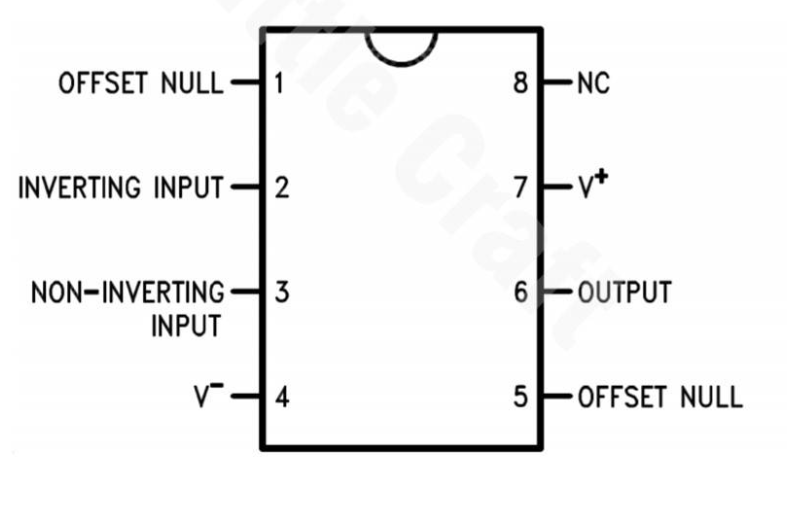
\includegraphics[width=0.6\linewidth]{figures/LM741.png}
	\caption{Schematische Skizze eines Operationsverstärkers und deren Anschlüsse \cite{LM741}.}
	\label{fig:OpAmp}
\end{figure}\noindent
Es wird zwischen einem idealen und einem realen Operationsverstärker unterschieden.
Ein idealer Operationsverstärker hat eine unendlich hohe Leerlaufverstärkung $V_\text{U}$, einen unendlich hohen Eingangswiderstand $R_\text{E}$ und einen Ausgangswiderstand von null.
Zudem besitzt er eine unendlich hohe Bandbreite und eine unendlich hohe Gleichtaktunterdrückung.
Ein realer Operationsverstärker hat lediglich eine Leerlaufleistung von $V_\text{U}\approx\SIrange{e4}{e7}{}$ und einen endlichen Eingangswiderstand von $R_\text{E}>\SI{1}{\mega\ohm}$ und einem Ausgangswiderstand von $R_\text{A}=\SIrange{10}{1000}{\ohm}$.
Die Bandbreite liegt zwischen $\SI{1}{\hertz}$ und $\SI{10}{\kilo\hertz}$.
Die Gleichtaktunterdrückung lässt sich bei einem realen OpAmp durch das Verhältnis aus Leerlaufverstärkung $V_0$ und Gleichtaktverstärkung $V_\text{G}$ beschreiben als
\begin{align}
    G=\frac{V_0}{V_G}.
\end{align}
Die Verstärkung des Amplifiers $A$ und die Bandbreite $BW$ stehen über das Gain-Bandwidth-Product $GBP$ über
\begin{align}
    GBP=A\cdot BW
\end{align}
im Zusammenhang.
Bei einer niedrigen Verstärkung kann der OpAmp effektiver über einen größeren Frequenzbereich eingesetzt werden.
Bei hohen Frequenzen kann der Verstärker keine stabile Verstärkung mehr liefern, da interne Kapazitäten und endliche Geschwindigkeiten der Komponenten die Verstärkung beeinflussen. \newline
Um mit einem OpAmp analoge Signale verarbeiten zu können, die sowohl positive, als auch negative Komponenten enthalten, werden zwei Versorgungsspannungen benötigt.
Damit diese eine gleichmäßige Ausgabe ermöglichen und unerwarteten Offets vorbeugen, werden die beiden Spannungen symmetrisch um die Nullspannung, meist $\pm U_\text{B}=\SI{15}{\volt}$, gewählt.
Dadurch ist die Amplitude des Ausgangssignals 
\begin{align}
    U_\text{A}=V\cdot(U_+-U_-),
    \label{eq:Amplitude_Ausgangssignal}
\end{align}
auf den Bereich $U_\text{A}\in[-U_\text{B},+U_\text{B}]$ beschränkt.
Ein Vorteil von zwei Versorgungsspannungen ist die \textit{common mode suppression}.
Als \textit{common mode} wird ein durchschnittliches Signal bezeichnet, das auf beiden Eingängen des OpAmps anliegt, also $V_{CM}=\sfrac{V_++V_-}{2}$.
Verstärkt wird nur die Differenz der beiden Eingangssignale, also $V_{\text{out}}=A\cdot(V_+-V_-)$, während idealerweise die Spannung $V_{CM}$ vollständig unterdrückt wird.
Bei idealen Operationsverstärkern ist dies der Fall, während bei realen OpAmps auch Teile des \textit{common mode} Signals verstärkt werden.\newline


\subsection{Grundlegende Schaltungen}\label{subsec:Grundlegende Schaltungen}        %%%%%%%%%%%%%%%% Grundlegende Schaltungen %%%%%%%%%%%%%%%%%%%%%
Durch Rückkopplung des Ausgangssignals auf den Eingang (Feedback) kann ein Operationsverstärker in Schaltungen mit unterschiedlichen Funktionen verwendet werden. 
Es wird dabei zwischen positivem Feedback, das das Eingangssignal verstärkt und negativem Feedback, das das Eingangssignal abschwächt, unterschieden.
In diesem Versuch werden die Schaltungen des invertierenden und nicht-invertierenden Linearverstärkers, des Integrators, des Differenzierers, des Schmitt-Triggers und des Generators untersucht.

\subsubsection{Der Invertierende Linearverstärker}\label{subsubsec:Invertierender Linearverstärker}
Ein invertierender Linearverstärker ist eine Schaltung, bei der das Eingangssignal auf den invertierenden Eingang (Gegenkopplung) gelegt wird.
Ein Schaltplan einer solchen Schaltung ist in \autoref{fig:inverting-OpAmp} dargestellt.
Um die Verstärkung zu berechnen, wird mithilfe von Gleichung (\ref{eq:Amplitude_Ausgangssignal}) und der Relation $U_0\equiv U_\text{A}$ die Ausgangsspannung am $i$-ten Knoten
\begin{align}
    U_i=-\frac{U_\text{A}}{V}.
\end{align}
Aufgrund der Kirchhoff'schen Knotenregel ergibt sich nun für den Knoten vor dem invertierten Eingang
\begin{align}
    \frac{U_i-U_1}{U_\text{A}-U_1} = \frac{R_1}{R_1+R_2},
\end{align}
woraus die Verstärkung
\begin{align}
    \label{eq:Verstärkung}
    \frac1{V'}&=-\frac{U_1}{U_\text{A}}=\frac{1}{V}+\frac{R_1}{R_2}\left(1+\frac{1}{V}\right),\quad |V\gg 1 \\
    \iff V' &\approx\frac{R_2}{R_1}\left(=\frac{U_\text{A}}{U_\text{E}}\right).
\end{align}
Die Bandbreite des Verstärkers wird um den folgenden Faktor erhöht
\begin{align}
    g\coloneqq\frac{V}{V'}.
\end{align}
\begin{figure}[H]
	\centering
    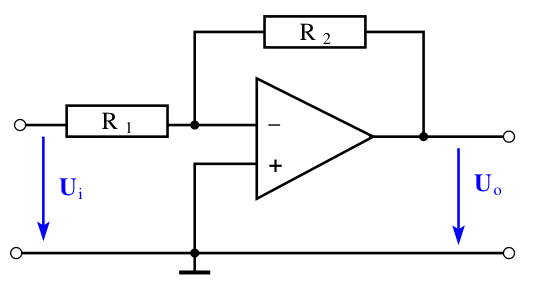
\includegraphics[width=0.6\linewidth]{figures/inverting-OpAmp.png}
	\caption{Elektrischer Schaltplan eines invertierenden Linearverstärkers \cite{Anleitung51}.}
	\label{fig:inverting-OpAmp}
\end{figure}

\subsubsection{Der Integrator}\label{subsubsec:Integrator}              %%%%%%%%%%%%%%%% Integrator %%%%%%%%%%%%%%%%%%%%%

Die Grundschaltung des Integrators ist ein invertierender Verstärker, der jedoch anstelle des Widerstandes $R_2$ einen Kondensator $C$ verwendet.
In \autoref{fig:integrator} ist der Schaltplan eines Integrators dargestellt.
Da die Ausgangsspannung $U_\text{A}$ im Zusammenhang mit der Ladungsmenge $Q$ des Kondensators $C$ steht, kann die Ausgangsspannung als Integral der Eingangsspannung $U_1$ über die Zeit $t$ beschrieben werden und wird somit als Integrator bezeichnet.
Hier gilt für den Strom $I_1$ aufgrund des Ohm'schen Gesetzes
\begin{align}
    \label{eq:OhmschesGesetz}
    I_1=-\frac{U_1}{R}
\end{align}
mithilfe von der Relation aus dem Knotenpunkt $I_1+I_C=0$ der folgende Ausdruck
\begin{align}
    \label{eq:StromKondensator}
    \int I_c\text dt=Q=CU_\text{A}.
\end{align}
Somit ergibt sich für die Ausgangsspannung
\begin{align}
    \label{eq:AusgangsspannungIntegrator}
    U_\text{A}=-\frac1{RC}\int U_1\text dt.
\end{align}
Für eine Wechselspannung $U_1=U_0\sin(\omega t)$ mit der Frequenz $\omega$ und der Amplitude $U_0$  folgt demnach
\begin{align}
    \label{eq:AusgangsspannungIntegratorWechselspannung}
    U_\text{A}=\frac{U_0}{\omega RC}\cos(\omega t).
\end{align}
Ein Integrator wird bei niedrigen Frequenzen verwendet, da niedrige Frequenzanteile stärker integriert werden können und somit einen größeren Einfluss auf die Ausgangsspannung haben.
Bei hohen Frequenzen nimmt die Verstärkung ab.
\begin{figure}[H]
	\centering
    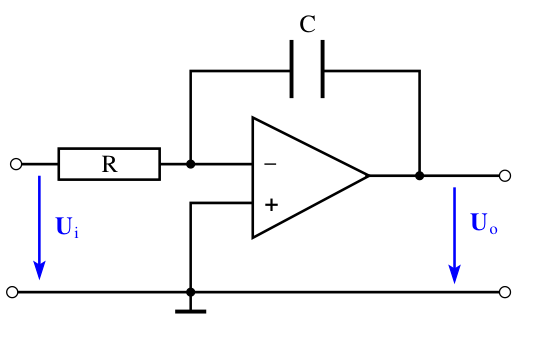
\includegraphics[width=0.6\linewidth]{figures/Integrator.png}
	\caption{Elektrischer Schaltplan eines Integrators \cite{Anleitung51}.}
	\label{fig:integrator}
\end{figure}


\subsubsection{Der Differenzierer}\label{subsubsec:Differenzierer}        %%%%%%%%%%%%%%%% Differenzierer %%%%%%%%%%%%%%%%%%%%%
Der Differenzierer ist in der Schaltung ein Integrator, bei dem der Kondensator $C$ und der Widerstand $R$ vertauscht sind.
In \autoref{fig:Differentiator} ist der Schaltplan eines Differenzierers dargestellt.
Aus der Beziehung zwischen Ladungsmenge $Q$ und Spannung $U$ des Kondensators $C$ folgt für die Spannung $U_\text{A}$ ein differenzierter Ausdruck, weshalb die Schaltung als Differenzierer bezeichnet wird.
Es folgt für die Ausgangsspannung
\begin{align}
    I_1 &= \dot Q = C\dot U_1, \\
    U_\text{A} &= -RC\dot U_1.
\end{align}
Am Beispiel einer sinusförmigen Wechselspannung $U_1=U_0\sin(\omega t)$ mit der Frequenz $\omega$ und der Amplitude $U_0$ ergibt sich für die Ausgangsspannung demnach
\begin{align}
    U_\text{A} = -\omega RCU_0\cos(\omega t).
\end{align}
\begin{figure}[H]
	\centering
    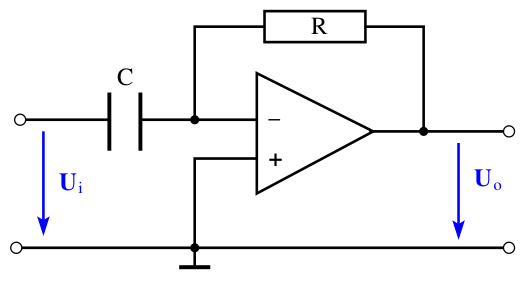
\includegraphics[width=0.6\linewidth]{figures/Differentiator.png}
	\caption{Elektrischer Schaltplan eines Differetiators \cite{Anleitung51}.}
	\label{fig:Differentiator}
\end{figure}


\subsubsection{Der Schmitt-Trigger}\label{subsubsec:Schmitt-Trigger}    %%%%%%%%%%%%%%%% Schmitt-Trigger %%%%%%%%%%%%%%%%%%%%%
Die grundlegende Schaltung eines Schmitt-Triggers ist in \autoref{fig:Schmitt-Trigger} dargestellt und unterscheidet sich von einem invertierenden Linearverstärker durch die Rückkopplung des Ausgangssignals auf den nicht-invertierenden Eingang, anstatt auf den invertierenden Eingang.
Dadurch wird eine Hysterese erzeugt, die dazu führt, dass das Ausgangssignal nur bei Überschreiten eines Schwellenwertes $U_\text{P}$ umschaltet.
Die Schaltung wird als Schmitt-Trigger bezeichnet, da sie ein Schaltsignal erzeugt, das bei Überschreiten eines Schwellenwertes umschaltet.
Die Schwellspannung kann mithilfe von
\begin{align}
    \label{eq:schmitt}
    U_\pm = \pm\frac{R_1}{R_2}U_\text{B}
\end{align}
mit der Sättigungsspannung des Operationsverstärkers $U_B$ berechnet werden, wobei ein überschreiten eines Wertes zum Umschalten des Ausgangssignals auf den Maximalwert und ein Unterschreiten auf den Minimalwert des Schmitt-Triggers führt.
Dies wird erst durch die Einführung der Hysterese möglich, die durch die positive Rückkopplung des Ausgangssignals auf den nicht-invertierenden Eingang erzeugt wird und somit erst dazu führt, dass ein maximaler/minimaler Wert angenommen wird.
Ohne die Hysterese würde der Schmitt-Trigger bereits bei geringen Schwankungen des Eingangssignals umschalten und somit oszillieren.
Die Ausgangsspannung eines Schmitt-Triggers ist immer eine Rechteckspannung.
Ein Differentiator, wird im Gegensatz zum Integrator, bei hohen Frequenzen eingesetzt, da hohe Frequenzanteile stärker differenziert werden können und somit einen größeren Einfluss auf die Ausgangsspannung haben.
Niedrige Frequenzen werden vom Differentiator nicht so gut angesprochen und sind durch Rauscheffekten gar problematisch.
\begin{figure}[H]
	\centering
    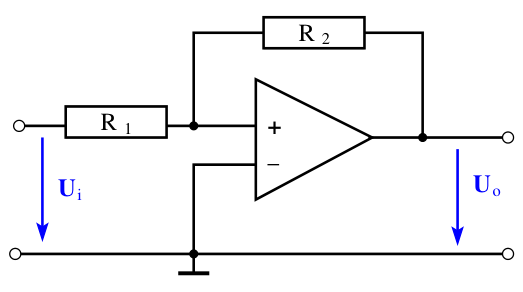
\includegraphics[width=0.6\linewidth]{figures/Schmitt-Trigger.png}
	\caption{Elektrischer Schaltplan eines Schmitt-Triggers \cite{Anleitung51}.}
	\label{fig:Schmitt-Trigger}
\end{figure}


\subsubsection{Der Generator}\label{subsubsec:Generator}                    %%%%%%%%%%%%%%%% Generator %%%%%%%%%%%%%%%%%%%%%
Wird ein Schmitt-Trigger mit einem Integrator kombiniert, dann entsteht ein Generator.
Ein Schaltplan eines Generators ist in \autoref{fig:Generator_einzeln} dargestellt.
Die Rechteckspannung des Schmitt-Triggers wird durch den Integrator in eine Dreieckspannung umgewandelt und dann wiederum auf den Eingang des Schmitt-Triggers zurückgeführt.
Dadurch entsteht ein periodisches Signal mit Frequenz $\nu_a$, die durch 
\begin{align}
    \label{eq:generator}
    \nu_a &= \frac{R_2}{4CR_1R_3}, \\
    U_1 &= U_{\text{B}}\frac{R_1}{R_2},
\end{align}
beschrieben werden kann.
Während bei einem solchen Generator das Schwingverhalten erst angeregt durch Ein- und Ausschalten angeregt werden muss, kann ein Generator mit variierender Amplitude auch ohne externe Anregung schwingen.
Ein Schaltplan eines solchen Generators ist in \autoref{fig:Generator-varyingAmplitudes} aufgezeichnet.
Das Schwingungsverhalten dieses Generators kann über die Differentialgleichung eines gedämpften harmonischen Oszillators beschrieben werden,
\begin{align}
    \label{eq:DGLGenerator}
    \frac{\text d^2U_\text{A}}{\text dt^2}-\frac{\eta}{10RC}\frac{\text dU_\text{A}}{\text dt}+\frac{1}{(RC)^2}U_\text{A}=0.
\end{align}
Dabei ist $\eta\in[-1,1]$ der Dämpfungsfaktor, der über $R_1$ einstellbar ist.
Wird $\eta<0$ gewählt, so wird der Generator zum Schwingkreis, der eine gedämpfte Schwingung erzeugt.
Bei $\eta>0$ oszilliert er.
Die Periodendauer $T$ des Schwingkreises ist durch
\begin{align}
    \label{eq:PeriodendauerGenerator}
    T=2\pi RC
\end{align}
und die Zerfallskonstante durch 
\begin{align}
    \tau=\frac{20RC}{|\eta|}
\end{align}
gekennzeichnet.
\begin{figure}[H]
	\centering
    \begin{subfigure}{\textwidth}
        \centering
        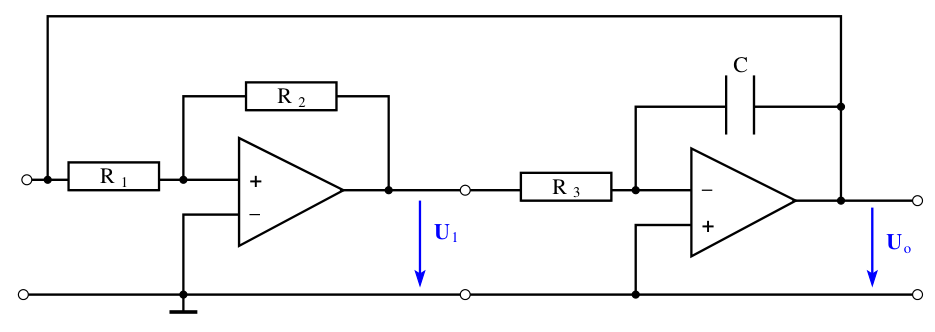
\includegraphics[width=0.8\linewidth]{figures/Generator.png}
        \caption{}
        \label{fig:Generator_einzeln}
    \end{subfigure}
    \begin{subfigure}{\textwidth}
        \centering
        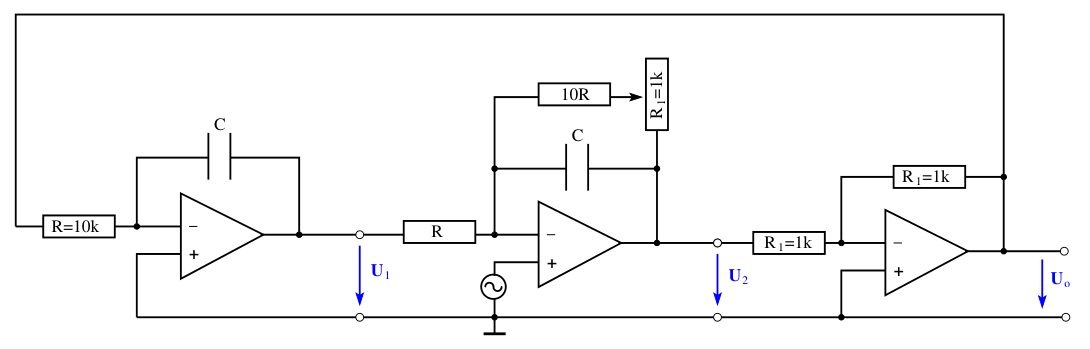
\includegraphics[width=0.8\linewidth]{figures/Generator-varyingAmplitudes.png}
        \caption{}
        \label{fig:Generator-varyingAmplitudes}
    \end{subfigure}
    \caption{Elektrischer Schaltplan zweier Generatoren \cite{Anleitung51}.}
    \label{fig:Generator}
\end{figure}

% \begin{figure}
%     \centering
%     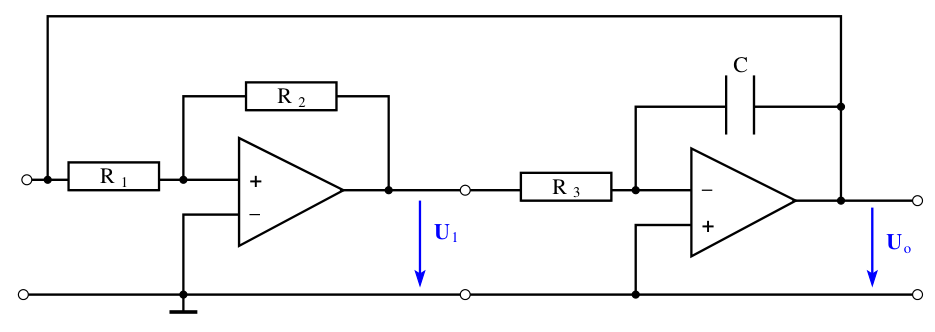
\includegraphics[width=0.6\linewidth]{figures/Generator.png}
%     \caption{Elektrischer Schaltplan eines Generator \cite{Anleitung51}.}
%     \label{fig:Generator}
% \end{figure}

% \begin{figure}
%     \centering
%     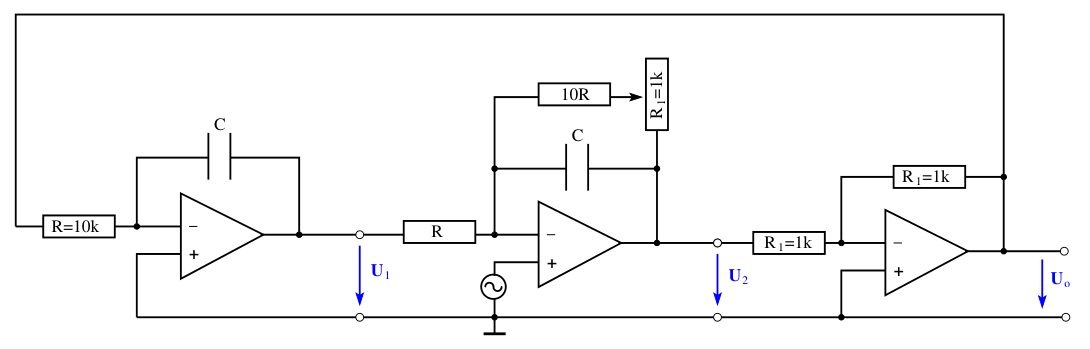
\includegraphics[width=0.6\linewidth]{figures/Generator-varyingAmplitudes.png}
%     \caption{Elektrischer Schaltplan eines Generator mit variierenden Amplituden \cite{Anleitung51}.}
%     \label{fig:Generator-varyingAmplitudes}
% \end{figure}